\chapter{Graphs}

\section{Graphs and Their Representation}

\begin{ans}
First, since $G$ is simple, we have $E(G) \subseteq \binom{V(G)}{2}$. That is, the edge set of $G$ is a subset of the set of unordered pairs of the elements of $V(G)$. We know that $\binom{|V(G)|}{2} = \binom{n}{2}$ counts the number of such unordered pairs, hence it follows that $m \le \binom{n}{2}$. We must have equality when all unordered pairs of vertices are in the edge set. This occurs in a complete graph.
\end{ans}

\begin{ans} \
\begin{itemize}
	\item[(a)] We will present a procedure for placing the edges between vertices to obtain the result. We begin with $n$ vertices in a bipartition $(X,Y)$ with $|X| = r$ and $|Y| = s$. Now for each vertex $v \in X$, we may place at most $s$ edges between $v$ and all vertices in $Y$ since $G$ is simple. So we may place at most $\underbrace{s + s + ... + s}_\text{$r$ times} = rs$ edges between the sets in the bipartition.
	\item[(b)] We have $r + s = n$ since $(X,Y)$ is a bipartition. If $n$ is even, we obtain the maximum number of edges in $G$ when $r = s = \frac{n}{2}$. So by part (a) we have $m \le \frac{n}{2} \cdot \frac{n}{2} = \frac{n^2}{4}$. If $n$ is odd, we obtain the maximum number of edges in $G$ when, without loss of generality, we have $r = \lceil\frac{n}{2}\rceil = \frac{n+1}{2}$ and $s = \lfloor\frac{n}{2}\rfloor = \frac{n-1}{2}$. So by part (b) we have $m \le \frac{n+1}{2} \cdot \frac{n-1}{2} = \frac{n^2 - 1}{4} \leq \frac{n^2}{4}$.
	\item[(c)] Equality holds when we have $|X| = |Y| = \frac{n}{2}$ for even $n = |V|$.
\end{itemize}
\end{ans}

\begin{ans} \
\begin{itemize}
	\item[(a)] Let $G$ be a path with $n = |V(G)|$. Then will create a path isomorphic to $G$ that is demonstrably bipartite. Consider the path $G' = (\{v_1,v_2,...,v_n\},\{v_1v_2,v_2,v_3,...,v_{n-1}v_n\})$. Then $(X,Y) = (\{v_i \in V(G'): \textrm{$i$ odd}\}, \{v_j \in V(G'): \textrm{$j$ even}\})$ is a bipartition of $G'$ since we only have odd indexed vertices adjacent to even indexed vertices, hence $G'$ is bipartite. Now we must present an isomorphism from $G$ to $G'$. Consider a function $\iota: V(G) \to V(G')$ where first $\iota$ maps an arbitrary endpoint of $G$ to an arbitrary endpoint of $G'$. We then construct $\iota$ by mapping a vertex $v \in V(G)$ to $v' \in V(G')$ if and only if $v$ is adjacent to $u \in V(G)$ such that $v'$ is adjacent to $\iota(u)$. By initialising this construction with only an endpoint, we have ensured that $\iota$ is a bijection under this rule and that $\iota$ preserves adjacency. Hence $\iota$ is an isomorphism. Thus we obtain that $G$ is bipartite under the bipartition $(X',Y') = (\{v \in V(G): \iota(v) \in X\},\{u \in V(G): \iota(u) \in Y\})$.
	\item[(b)] Let $G$ be a cycle. Assume $G$ is bipartite under the bipartition $(X,Y)$. Now suppose, towards a contradiction, that $G$ has odd length. Then $n$ is odd, since we may associate each edge in $G$ with a single vertex, so either $|X|$ or $|Y|$ is odd. Assume, without loss of generality, that $|X|$ is odd and $|Y|$ is even. We have that $d(v) = 2$ for all $v \in V(G)$, so counting all edges in $G$ from $X$ to $Y$, we have $2|X|$ edges in $G$. Clearly this is not odd, so we have a contradiction. Hence $G$ must have even length. Now assume that $G$ is a cycle with even length. Removing an arbitrary edge in $G$ produces a path of odd length, which is bipartite from part (a). We obtain our bipartition $(X,Y)$ using the method in (a) and then add in the previously removed edge. The endpoints of the path are in different parts of the partition, since there are an even number of vertices, so the extra edge is added between the parts, hence our bipartition is preserved. Thus, $G$ is bipartite. So we have that a cycle is bipartite if and only if it has even length.
\end{itemize}
\end{ans}

\begin{ans}
Let $G = (\{v_1,...,v_n\},E)$. For any vertex $u \in V(G)$, $\delta(G) \leq d_G(u)$ by definition, so we have $\delta(G) = \frac{n \cdot \delta(G)}{n} \leq \frac{d_G(v_1) + ... + d_G(v_n)}{n} = d(G)$. Similarly, for any vertex $u \in V(G)$, $d_G(u) \leq \Delta(G)$, so $d(G) = \frac{d(v_1) + ... + d(v_n)}{n} \leq \frac{n \cdot \Delta(G)}{n} = \Delta(G)$. Hence $\delta(G) \leq d(G) \leq \Delta(G)$.
\end{ans}

\begin{ans}
Let $G$ be a $k$-regular graph. If $k=0$, then we have no edges in $G$ since the degree of each vertex is 0. If $k=1$, then $G$ consists of any number of components of 2 vertices joined by an edge. If $k=2$, then $G$ consists of any number of components that are cycles.
\end{ans}

\begin{ans} \
\begin{itemize}
	\item[(a)] We represent this problem with a simple graph $G = (V,E)$ where the vertices represent people in the group and two vertices are adjacent if the represented people are friends. Hence we seek to prove that $d(u) = d(v)$ for distinct $u,v \in V$. Given a vertex $v \in V$, we must have $d(v) \in \{0,1,...,n-1\}$ since $G$ is simple. However, if there exists a vertex of degree 0 in $G$ then we cannot have a vertex of degree $n-1$ in $G$, and vice versa. Hence we have $n$ vertices in $G$ with only $n-1$ options for the degree of each vertex. Thus, by the pigeonhole principle there exist at least two vertices of $G$ with equal degree.
	\item[(b)] We present a graphic representation of the group of friends below.
	\begin{center}
		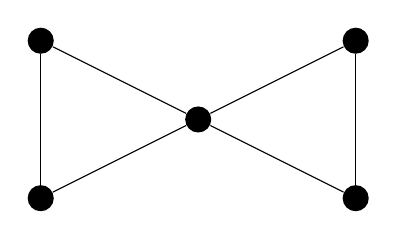
\begin{tikzpicture}
			\draw (0,0) node[fill=black, circle] (A) {};
			\draw (0,2) node[fill=black, circle] (B) {};
			\draw (2,1) node[fill=black, circle] (C) {};
			\draw (4,0) node[fill=black, circle] (D) {};
			\draw (4,2) node[fill=black, circle] (E) {};
			
			\draw (A) -- (B);
			\draw (A) -- (C);
			\draw (B) -- (C);
			\draw (C) -- (D);
			\draw (C) -- (E);
			\draw (D) -- (E);
		\end{tikzpicture}
	\end{center}
\end{itemize}
\end{ans}